\chapter{Antecedentes}
\label{chapter:antecedentes}

Este capítulo presenta los antecedentes necesarios para situar el problema abordado en este trabajo, desde la evolución de los sistemas de almacenamiento hasta las técnicas actuales de asignación de ubicaciones.
Comienza por la historia, desde el almacén que solo custodiaba mercadería hasta el \emph{warehouse} moderno que despacha miles de pedidos por día, y desde ahí baja a las operaciones que ocurren puertas adentro, con el foco puesto en el \emph{picking}.
Sobre ese terreno entra después la literatura sobre asignación de ubicaciones y sobre el uso de la afinidad entre productos, que es la que termina señalando los huecos que este trabajo está en posición de atacar.
Todo lo que sigue habla de centros de distribución en general, mientras que el que se estudió y los datos que se utilizaron se describen más adelante, en un capítulo propio\completar{poner la ref cuando el capitulo exista}.




\section{Evolución de los depósitos y centros de distribución}
\label{sec:evolucion}


Durante buena parte de su historia, un depósito fue principalmente un lugar donde la mercadería esperaba.

Los productos llegaban, se almacenaban y permanecían allí hasta que fueran necesarios. Esto permitía producir en un momento y vender en otro, algo especialmente importante cuando la demanda se concentraba en ciertas épocas del año. Un fabricante de juguetes, por ejemplo, podía producir durante varios meses y acumular stock para responder al aumento de ventas durante Navidad. Al mismo tiempo, mantener inventario daba cierto margen frente a cambios inesperados en la demanda.

Amortiguar el desfasaje entre producción y venta no es, sin embargo, el único motivo para sostener un depósito.
Hay otro menos evidente y de naturaleza casi aritmética, que es la consolidación del transporte \citep[sección~1.1]{bartholdi2014warehouse}.
Si $m$ proveedores deben abastecer directamente a $n$ comercios hacen falta del orden de $m \times n$ envíos, cada uno relativamente chico y por lo tanto caro por unidad transportada, mientras que si toda la mercadería pasa por un depósito intermedio alcanzan $m + n$ envíos, cada uno más grande y con el camión más lleno.
Con cien proveedores y cien comercios la diferencia es entre diez mil conexiones posibles y apenas doscientas a través de un punto intermedio. Esta capacidad de unificar flujos terminó siendo otra de las razones económicas para introducir depósitos en una cadena logística.
Concentrar la mercadería en un punto tiene además otras ventajas, como aprovechar descuentos por compra en volumen o postergar la configuración final de un producto genérico hasta saber qué mercado lo pide.

En ese contexto, la principal preocupación era encontrar espacio para guardar la mercadería y aprovecharlo bien. Como los productos se movían con menos frecuencia, la ubicación exacta de cada uno dentro del depósito tenía una importancia mucho menor que la que tiene en una operación moderna.


Ese equilibrio empezó a cambiar a medida que crecieron los volúmenes de producción y de mercadería almacenada. Ya no alcanzaba con disponer de espacio suficiente, también era necesario mover los productos dentro del depósito de forma cada vez más eficiente. Así, el problema comenzó a desplazarse
desde dónde guardar la mercadería hacia cómo manipularla y transportarla.

Una de las respuestas llegó por el lado de la estandarización, con la difusión de la carga unitaria a mediados del siglo~XX.
Un \emph{pallet} es una plataforma de medidas normalizadas sobre la que se apila mercadería para manipularla como un bloque único, y su adopción masiva, junto con la del montacargas, convirtió el movimiento de mercadería en una operación mecanizable y previsible.
Esta forma de manipular la mercadería también consolidó durante décadas una operación pensada alrededor de grandes unidades de carga, algo que cambiaría profundamente con la expansión del comercio electrónico.

Sobre esa base material se constituyó la logística como disciplina durante la segunda mitad del siglo.
Lo que hasta entonces eran actividades sueltas, almacenar, transportar, reponer, empezó a tratarse como un sistema con objetivos propios y costos medibles \citep{ballou2007evolution}.

Otro giro, conceptual antes que tecnológico, vino con la difusión de las filosofías de producción ajustada a partir de los años setenta.
Mantener grandes cantidades de inventario también tiene un costo, el mismo ocupa espacio, requiere recursos para su almacenamiento y queda expuesto a roturas, deterioro u obsolescencia. Por eso, el almacenamiento comenzó a verse no solo como un respaldo frente a la incertidumbre, sino también como capital inmovilizado y como una fuente de costos.

Las consecuencias para lo que aquí importa son dos.
Por un lado el depósito dejó de ser un lugar donde la mercadería descansa y pasó a ser uno donde circula, lo que vuelve al movimiento interno un costo mucho más importante en lugar de una externalidad menor.
Por otro lado, al aumentar la frecuencia de los movimientos, comenzó a cobrar importancia una característica hasta entonces menos relevante para organizar el espacio, qué productos se solicitaban con mayor frecuencia. Esa información podía utilizarse para ubicar los artículos de mayor rotación en posiciones más convenientes.

En ese contexto se consolidó la figura del centro de distribución, que se distingue del almacén tradicional menos por su tamaño que por aquello que mide.
Mientras que en el almacén tradicional la capacidad de almacenamiento ocupaba un lugar central, en un centro de distribución adquieren mayor importancia la cantidad de pedidos procesados, el tiempo necesario para hacerlo y el costo asociado a cada uno.

Hablar de centros de distribución, sin embargo, todavía abarca operaciones que se parecen poco entre sí, y la distinción más útil pasa por el tipo de cliente al que sirven \citep[sección~1.2]{bartholdi2014warehouse}.
Uno que abastece tiendas trabaja contra un cliente más regular y previsible, con órdenes que pueden tener cientos o miles de artículos y que suelen conocerse con un día o más de anticipación, de modo que hay margen para planificar.
Un depósito de repuestos enfrenta el problema opuesto, porque llega a almacenar decenas o cientos de miles de piezas cuya demanda individual es chica y difícil de anticipar, aunque la actividad en promedio resulte estable.
En el extremo opuesto está el centro de distribución orientado al comercio electrónico masivo, donde las órdenes suelen ser pequeñas, en muchas ocasiones de apenas uno a tres artículos, pero llegan con una frecuencia muy alta y deben procesarse rápidamente.
A eso se agregan operaciones con restricciones propias, como los depósitos de perecederos, en los que la mercadería permanece a veces solo unas horas y hay que sostener la cadena de frío y reglas de salida por vencimiento, o los operadores logísticos externos, que conviven en una misma instalación con inventario de varios clientes.
La Tabla~\ref{tab:tipos-deposito} resume estas diferencias, que van a reaparecer a lo largo del capítulo cada vez que una decisión dependa del tipo de operación.\completar{resta muy copiada asi nomas esta tabla, en uno de los libros habia una mejor }

\begin{table}[ht]
    \centering
    \small
    \begin{tabularx}{\textwidth}{|l|L|L|L|}
        \hline
        \textbf{Tipo} & \textbf{Cliente típico} & \textbf{Orden típica} & \textbf{Presión dominante} \\
        \hline
        Reposición de tiendas & comercios de una cadena & cientos o miles de artículos, conocida con anticipación & mover volumen según plan \\
        \hline
        Repuestos & talleres y equipos en servicio & pocas líneas, a menudo urgentes & variedad enorme, demanda difícil de anticipar \\
        \hline
        Comercio electrónico & consumidor final & uno a tres artículos & muchísimas órdenes chicas, despacho inmediato \\
        \hline
        Perecederos & comercios y consumidores & variable & permanencia corta, cadena de frío \\
        \hline
        Operador logístico & varios clientes a la vez & mixta & inventarios de distintos dueños conviviendo \\
        \hline
    \end{tabularx}
    \caption{Tipos de centro de distribución según el cliente al que sirven }
    \label{tab:tipos-deposito}
\end{table}

Esas diferencias no son solo de escala, porque también cambia la unidad física con la que se manipula la mercadería.
Cerca de la fábrica el producto tiende a moverse en \emph{pallets}, y a medida que avanza por la cadena de distribución esas grandes unidades se van dividiendo en cajas, paquetes internos y, finalmente, unidades individuales, que es la escala más cercana al consumidor final \citep[sección~2.2]{bartholdi2014warehouse}.

Conviene distinguir esa escala física de la identidad del producto.
Cada producto o variante que el inventario administra de manera independiente se identifica mediante una \emph{SKU}, sigla de \emph{stock keeping unit}, y una misma SKU puede estar presente a la vez en pallets, en cajas y en piezas sueltas, del mismo modo que dos variantes de un artículo, por talle o por color, son dos SKU distintas aunque físicamente casi no se diferencien.
La unidad suelta con la que termina la Figura~\ref{fig:unidades-manipulacion} es entonces lo más chico que el depósito manipula, mientras que la SKU es la referencia con la que lo cuenta, y de aquí en adelante se usa en ese sentido.

\begin{figure}[ht]
    \centering
    \begin{tikzpicture}[x=1cm, y=1cm, every node/.style={font=\small}]
        % pallet: pila de cajas sobre una base
        \foreach \i in {0,1,2}
            \foreach \j in {0,1,2}
                \draw[fill=gray!20, draw=black!70] (\i*0.63, \j*0.5) rectangle ++(0.58, 0.44);
        \draw[fill=gray!50, draw=black!70] (-0.08, -0.2) rectangle (1.92, -0.04);
        \node at (0.92, -0.65) {\emph{pallet}};
        \draw[-{Stealth}, thick, black!60] (2.25, 0.7) -- (2.95, 0.7);
        % caja con unidades adentro
        \foreach \i in {0,1}
            \foreach \j in {0,1}
                \draw[fill=gray!20, draw=black!70] (3.25+\i*0.46, 0.24+\j*0.46) rectangle ++(0.42, 0.42);
        \draw[draw=black!70, thick] (3.2, 0.19) rectangle (4.22, 1.21);
        \node at (3.71, -0.65) {caja};
        \draw[-{Stealth}, thick, black!60] (4.55, 0.7) -- (5.25, 0.7);
        % paquete interno: tira de unidades
        \foreach \i in {0,1,2}
            \draw[fill=gray!20, draw=black!70] (5.55+\i*0.36, 0.54) rectangle ++(0.32, 0.32);
        \draw[draw=black!70, thick] (5.5, 0.49) rectangle (6.66, 0.91);
        \node at (6.08, -0.65) {paquete interno};
        \draw[-{Stealth}, thick, black!60] (7.0, 0.7) -- (7.7, 0.7);
        % unidad suelta
        \draw[fill=gray!20, draw=black!70] (7.95, 0.54) rectangle ++(0.32, 0.32);
        \node at (8.11, -0.65) {unidad};
    \end{tikzpicture}
    \caption{La unidad de manipulación se reduce a medida que el producto avanza por la cadena de distribución.}
    \label{fig:unidades-manipulacion}
\end{figure}


Ese descenso es el que vuelve relevante todo lo que sigue.
Mover un pallet entero de una ubicación a otra es un problema distinto de recorrer el depósito para juntar una o dos unidades de varios productos diferentes, y cuanto más chica es la unidad que se manipula y más pedidos hay que preparar, más peso adquiere la decisión de dónde ubicar cada artículo.

\section{La digitalización y el warehouse moderno}
\label{sec:digitalizacion}

El aumento en la cantidad de productos, ubicaciones y movimientos hizo que muchos aspectos que antes parecían irrelevantes fueran cada vez más importantes, y al mismo tiempo volvió mucho más difícil administrar el depósito de forma manual.
Un centro de distribución grande puede ocupar decenas de miles de metros cuadrados, almacenar alrededor de cien mil productos distintos y emplear a cientos de personas que preparan miles de pedidos por día \citep[capítulo~4]{bartholdi2014warehouse}.

A esa escala ya no alcanza con conocer el depósito por experiencia o recordar dónde se encontraba cada producto, porque estas medidas requirieron un registro actualizado del inventario, de sus ubicaciones y de los movimientos que ocurren continuamente dentro de la instalación.
Parte de la respuesta a esa necesidad fue la incorporación progresiva de sistemas de información capaces de acompañar y coordinar la operación del depósito.


Los sistemas de gestión de almacenes, sin embargo, no empiezan por ahí.
Su capacidad más básica es registrar la entrada y la salida de mercadería, por una razón contable antes que operativa, ya que la recepción de productos dispara el pago a los proveedores mientras que la salida dispara la facturación al cliente \citep[sección~4.1]{bartholdi2014warehouse}.
Sobre esa base se fue construyendo todo lo demás.

El siguiente salto de funcionalidad consiste en registrar no solo cuánto inventario queda sino también dónde está, es decir, administrar un inventario de ubicaciones además de uno de productos.
Eso es lo que la literatura llama \emph{stock locator system}, y es lo que le permite al software dejar de limitarse a transacciones contables para dirigir la operación diaria \citep[sección~4.2]{bartholdi2014warehouse}.
Con esa información el sistema puede dirigir tanto el \emph{put-away}, indicando dónde guardar cada SKU, como el picking, indicando de dónde retirarla, y sobre esa misma representación del almacén se apoyan funciones cada vez más amplias, desde coordinar reposiciones hasta distribuir trabajo entre los operarios.

Con esas capacidades, procesar un pedido ya no exige recorrer sus productos en el orden en que el cliente los pidió.
El propio sistema recibe las órdenes y las transforma en una lista de recolección reordenada por conveniencia, del mismo modo en que alguien que llega al supermercado con una lista de cosas que comprar la reagrupa mentalmente antes de hacer el recorrido, y es esa lista, y no la memoria del operario, la que le indica qué ubicaciones visitar.

Sostener ese control exigió que registrar dejara de ser una tarea aparte.
Con la difusión del código de barras a partir de los años setenta, identificar un producto o una ubicación dejó de requerir transcripción manual \citep{brown1997revolution}, y como cada lectura ocurre en el momento y en el lugar del movimiento que registra, el inventario del sistema pudo acercarse mucho más al estado real del depósito.
Ese acercamiento no lo logra el código por sí solo, porque hace falta además que las terminales acompañen al operario hasta donde ocurre el movimiento, que la base de datos absorba actualizaciones simultáneas desde recepción, picking y despacho, y que los procedimientos obliguen a escanear en cada paso \citep[sección~4.2]{bartholdi2014warehouse}.
Cuando todo eso está, el nivel de detalle es fino, al punto de que un buen WMS rastrea cada lugar donde puede haber producto, incluidas las horquillas de cada montacargas.

El alcance de estos sistemas sigue creciendo, y el WMS se relaciona con los sistemas del resto de la empresa, de los que recibe las órdenes y a los que devuelve un resumen de lo que ocurre puertas adentro, integrado en la planificación de la cadena de suministro completa \citep[capítulo~4]{bartholdi2014warehouse}.
Ese control es una de las razones por las que la cadena de suministro se aceleró tanto entre los años noventa y la década de 2010, y para dar una idea del cambio basta recordar que hasta no hace tanto cualquier compra por catálogo venía acompañada de la advertencia de que la entrega podía demorar entre seis y ocho semanas, algo que hoy resultaría inaceptable \citep[capítulo~4]{bartholdi2014warehouse}.
El argumento de los autores es que un producto controlado con precisión se mueve más rápido y con menos inventario en el sistema, una mejora que se suma a las del transporte y de la coordinación entre eslabones.

A esto se suma una consecuencia que va a reaparecer a lo largo de todo el capítulo.
Para poder realizar todas estas tareas, el sistema está obligado a registrar cada movimiento, de modo que el depósito termina acumulando el historial completo de qué se pidió, cuándo, en qué cantidad y junto con qué otra cosa.
Ese registro, que nadie arma a propósito sino que se genera solo como consecuencia de la operación diaria, termina siendo la materia prima sobre la que se apoya buena parte de la literatura que se revisa en este capítulo.


Fue sobre esa base informatizada que aterrizó el cambio de demanda descripto en la sección anterior.
A ese cambio de escala el comercio electrónico le sumó complicaciones que hasta entonces eran marginales, ya que una parte de lo despachado empezó a volver en forma de devoluciones y una misma instalación pasó a atender varios canales a la vez, reponiendo tiendas y despachando a clientes finales desde el mismo edificio, aunque los dos tipos de pedido se parezcan poco \citep{boysen2019warehousing}.
Las devoluciones en particular invirtieron el sentido del flujo, porque cada paquete que vuelve tiene que ser recibido, controlado y guardado otra vez con el mismo cuidado que un producto recién llegado del proveedor, con la diferencia de que llega de a una unidad, en un estado que nadie conoce de antemano y sin que ningún plan lo haya previsto.

\completar{PENDIENTE 2.2: dos parrafos antes del cierre para equilibrar el gradiente temporal, (a) la automatizacion como historia, AS/RS, carruseles, robots moviles y Kiva 2012 (L 12.3, Boysen 2019), el capital como tercer costo; (b) el deposito moderno no es uno solo, contrastes regionales del cap 16 de L, Norteamerica y Amazon, China, India, Singapur, y decidir si entra Sudamerica. Despues reescribir el cierre para que no repita.}
La industria ensayó respuestas muy distintas a esa presión, desde automatizar el movimiento interno hasta repensar la organización del trabajo y del espacio, y buena parte de las secciones que siguen está dedicada a recorrerlas.

\section{Operaciones dentro de un warehouse}
\label{sec:operaciones}

En las secciones anteriores la operación del depósito apareció varias veces, pero siempre de costado, como telón de fondo de la historia o de los sistemas que la coordinan.
Ahora bien, para optimizar cualquiera de las decisiones que se toman puertas adentro es necesario entender primero esas operaciones en detalle, y la manera más natural de hacerlo es seguir el camino que recorre la mercadería desde que baja de un camión hasta que sale despachada hacia un cliente.
Esta sección recorre ese camino preguntándose en cada etapa qué cuesta y dónde se decide ese costo, junto con el edificio y el equipamiento donde todo ocurre, hasta desembocar en la etapa que se lleva la mayor parte, el \emph{order picking}.

\subsection{Dónde se decide el costo}

\begin{figure}[ht]
    \centering
    \begin{tikzpicture}[node distance=0.3cm, box/.style={draw=black!70, fill=gray!12, rounded corners=2pt, minimum height=0.8cm, inner xsep=4pt, font=\footnotesize}]
        \node[box] (r) {recepción};
        \node[box, right=of r] (p) {put-away};
        \node[box, right=of p] (a) {almacenamiento};
        \node[box, right=of a] (k) {picking};
        \node[box, right=of k] (e) {empaque};
        \node[box, right=of e] (d) {despacho};
        \foreach \x/\y in {r/p, p/a, a/k, k/e, e/d} \draw[-{Stealth}, black!60] (\x) -- (\y);
    \end{tikzpicture}
    \caption{Las etapas que recorre la mercadería dentro de un warehouse.}
    \label{fig:flujo-operaciones}
\end{figure}

El recorrido empieza y termina en el \emph{dock}, la zona del depósito donde se desarman las cargas que llegan y, más tarde, se arman las que salen, de modo que casi todo lo que entra y sale pasa por ahí \citep[capítulo~3]{bartholdi2014warehouse}.
La mercadería que se descarga llega todavía en las unidades grandes de la Sección~\ref{sec:evolucion}, pallets o cajas cerradas, y por eso recibirla exige comparativamente poco trabajo por unidad.

Una parte importante del costo posterior se condiciona un paso más adelante, en el \emph{put-away}.
Antes de guardar hay que elegir dónde, y de esa elección depende en buena medida cuánto habrá que caminar después para volver a buscar cada producto, de modo que una etapa fija un costo que otra paga.
Por otro lado, en la espera a que algún pedido solicite una SKU, la mercadería no consume trabajo pero sí espacio, ocupando una ubicación con dirección propia dentro del depósito.

Del lado de la salida, lo recolectado pasa por el control y el empaque antes de volver al dock, y ahí detectar un error todavía es barato, porque un pedido mal despachado cuesta el envío de vuelta, el reproceso y un cliente decepcionado.

Una regla atraviesa todas las etapas, y es que el producto fluya deteniéndose lo menos posible, porque cada vez que un bulto se deja en algún lugar intermedio alguien va a tener que volver a levantarlo, y esa doble manipulación, sumado sobre los cientos de miles de piezas que pasan por un depósito, se vuelve un costo considerable.

La Tabla~\ref{tab:costos-etapas} le pone números a ese reparto.
Son estimaciones típicas reportadas en la literatura clásica de planificación de instalaciones, y conviene leerlas como órdenes de magnitud antes que como medidas, porque la proporción exacta depende de qué se almacena y a quién se atiende, mientras que el orden entre las etapas se mantiene en casi todos los casos reportados \citep{tompkins2010facilities, dekoster2007design}.

\begin{table}[ht]
    \centering
    \begin{tabular}{|l|c|}
        \hline
        \textbf{Etapa} & \textbf{Participación en el costo operativo} \\
        \hline
        Recepción & 10\% \\
        \hline
        Put-away & 15\% \\
        \hline
        Order picking & 55\% \\
        \hline
        Control, empaque y despacho & 20\% \\
        \hline
    \end{tabular}
    \caption{Reparto típico del costo operativo entre etapas, según las estimaciones clásicas de \citet{tompkins2010facilities} reproducidas en \citet[capítulo~3]{bartholdi2014warehouse}.}
    \label{tab:costos-etapas}
\end{table}

\subsection{El edificio como variable}

La geometría de un warehouse es de las decisiones más difíciles de revertir, porque se fija al construir el edificio y sus consecuencias permanecen durante décadas.
El esquema dominante es sencillo, con la superficie dividida en pasillos paralelos flanqueados por estanterías más el dock, y la Figura~\ref{fig:geometrias} muestra esa forma básica junto con sus variantes principales.
Sobre esa base, cada elección de diseño es en el fondo un problema de optimización cuyas consecuencias se pagan o se cobran en cada recorrido posterior.

Una de esas elecciones es cuántos docks tener y dónde ponerlos, y su efecto es menos obvio de lo que parece, porque no cambia cuánto espacio hay sino cómo se reparte la conveniencia entre las ubicaciones \citep[sección~6.2]{bartholdi2014warehouse}.
Cuando la recepción y el despacho comparten un mismo dock, en la configuración conocida como flujo en U de la Figura~\ref{fig:geo-u}, unas pocas ubicaciones cercanas quedan muy convenientes y las esquinas opuestas quedan muy castigadas, mientras que si hay un dock de entrada y otro de salida en lados opuestos, en el flujo pasante de la Figura~\ref{fig:geo-pasante}, el producto cruza el edificio y muchas ubicaciones resultan igual de razonables, aunque ninguna excepcional.
Ninguna de las dos configuraciones domina a la otra, y el criterio es elegir según el sesgo de la demanda, porque una operación donde pocas SKU concentran la actividad aprovecha mejor el puñado de posiciones excelentes del flujo en U, mientras que una de actividad más repartida prefiere la uniformidad del flujo pasante.
El patrón del argumento es lo más valioso que deja esta elección: la geometría define qué ubicaciones valen más, y la demanda define cuánto conviene esa definición.

Los pasillos admiten sus propias variantes.
En general conviene orientarlos en la dirección del flujo, y es habitual agregar pasillos transversales que permiten cortar camino entre ubicaciones, como en la Figura~\ref{fig:geo-transversal}, al precio de resignar posiciones de almacenamiento y de alargar levemente los viajes que los cruzan.
Se ha propuesto incluso abandonar el paralelismo, porque reorientar algunos pasillos en diagonal hacia el dock, en la espina de pescado de la Figura~\ref{fig:geo-espina}, acorta el viaje entre un punto central de despacho y cada ubicación, con reducciones de hasta un 20\% en depósitos de carga unitaria, donde cada viaje es de ida y vuelta a una sola ubicación, a cambio de un edificio algo más grande \citep{gue2009aisle}.
Esa ventaja se achica cuando un mismo recorrido visita muchas ubicaciones, pero que un cambio de ángulo pueda mover tanto la cuenta da una idea de cuánto pesan decisiones que parecen puramente arquitectónicas.

\begin{figure}[ht]
    \centering
    \begin{subfigure}{0.48\textwidth}
        \centering
        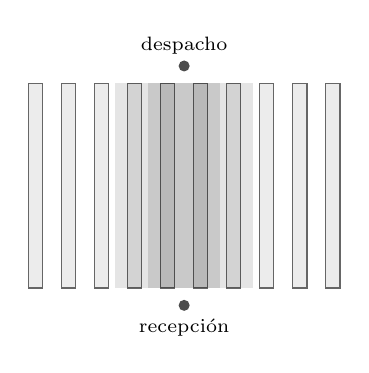
\begin{tikzpicture}[x=1cm, y=1cm]
            \foreach \i in {0,...,9} \draw[fill=gray!15, draw=black!60] (\i*0.42, 0) rectangle ++(0.18, 2.6);
            \fill[black, opacity=0.10] (1.10, 0) rectangle (2.86, 2.6);
            \fill[black, opacity=0.12] (1.52, 0) rectangle (2.44, 2.6);
            \fill[black!70] (1.98, -0.22) circle (0.07);
            \fill[black!70] (1.98, 2.82) circle (0.07);
            \node[font=\scriptsize] at (1.98, -0.5) {recepción};
            \node[font=\scriptsize] at (1.98, 3.08) {despacho};
        \end{tikzpicture}
        \caption{flujo pasante}
        \label{fig:geo-pasante}
    \end{subfigure}
    \hfill
    \begin{subfigure}{0.48\textwidth}
        \centering
        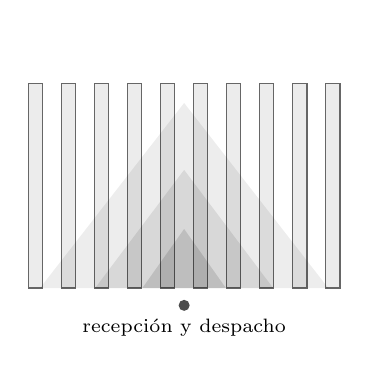
\begin{tikzpicture}[x=1cm, y=1cm]
            \foreach \i in {0,...,9} \draw[fill=gray!15, draw=black!60] (\i*0.42, 0) rectangle ++(0.18, 2.6);
            \fill[black, opacity=0.07] (1.98, 2.35) -- (0.15, 0) -- (3.81, 0) -- cycle;
            \fill[black, opacity=0.09] (1.98, 1.5) -- (0.85, 0) -- (3.11, 0) -- cycle;
            \fill[black, opacity=0.12] (1.98, 0.75) -- (1.45, 0) -- (2.51, 0) -- cycle;
            \fill[black!70] (1.98, -0.22) circle (0.07);
            \node[font=\scriptsize] at (1.98, -0.5) {recepción y despacho};
            \node[font=\scriptsize, opacity=0] at (1.98, 3.08) {despacho};
        \end{tikzpicture}
        \caption{flujo en U}
        \label{fig:geo-u}
    \end{subfigure}

    \vspace{0.8em}

    \begin{subfigure}{0.48\textwidth}
        \centering
        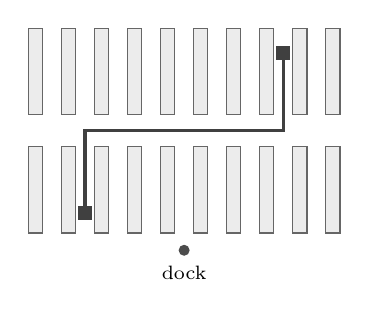
\begin{tikzpicture}[x=1cm, y=1cm]
            \foreach \i in {0,...,9} {
                \draw[fill=gray!15, draw=black!60] (\i*0.42, 1.5) rectangle ++(0.18, 1.1);
                \draw[fill=gray!15, draw=black!60] (\i*0.42, 0) rectangle ++(0.18, 1.1);
            }
            \draw[very thick, black!75] (0.72, 0.3) -- (0.72, 1.3) -- (3.24, 1.3) -- (3.24, 2.25);
            \fill[black!75] (0.63, 0.16) rectangle ++(0.18, 0.18);
            \fill[black!75] (3.15, 2.2) rectangle ++(0.18, 0.18);
            \fill[black!70] (1.98, -0.22) circle (0.07);
            \node[font=\scriptsize] at (1.98, -0.5) {dock};
        \end{tikzpicture}
        \caption{pasillo transversal}
        \label{fig:geo-transversal}
    \end{subfigure}
    \hfill
    \begin{subfigure}{0.48\textwidth}
        \centering
        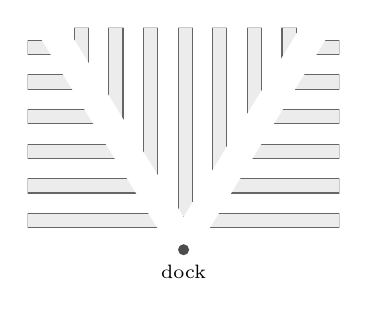
\begin{tikzpicture}[x=1cm, y=1cm]
            \begin{scope}
                \clip (0, 0) -- (1.68, 0) -- (0.08, 2.6) -- (0, 2.6) -- cycle;
                \foreach \j in {0,...,5} \draw[fill=gray!15, draw=black!60] (0, 0.06+\j*0.44) rectangle (1.9, 0.24+\j*0.44);
            \end{scope}
            \begin{scope}
                \clip (2.28, 0) -- (3.96, 0) -- (3.96, 2.6) -- (3.88, 2.6) -- cycle;
                \foreach \j in {0,...,5} \draw[fill=gray!15, draw=black!60] (2.0, 0.06+\j*0.44) rectangle (3.96, 0.24+\j*0.44);
            \end{scope}
            \begin{scope}
                \clip (1.98, 0.2) -- (0.5, 2.6) -- (3.46, 2.6) -- cycle;
                \foreach \k in {0,...,8} \draw[fill=gray!15, draw=black!60] (0.15+\k*0.44, 0.2) rectangle ++(0.18, 2.4);
            \end{scope}
            \fill[black!70] (1.98, -0.22) circle (0.07);
            \node[font=\scriptsize] at (1.98, -0.5) {dock};
        \end{tikzpicture}
        \caption{espina de pescado}
        \label{fig:geo-espina}
    \end{subfigure}
    \caption{Variantes de geometría de un depósito. La ubicación de los docks y la orientación de los pasillos cambian qué ubicaciones resultan convenientes, y en (a) y (b) el sombreado más oscuro indica mayor conveniencia. Esquemas adaptados de \citet[capítulo~6]{bartholdi2014warehouse}.}
    \label{fig:geometrias}
\end{figure}

El equipamiento que llena esa geometría responde siempre a alguno de dos propósitos, ahorrar trabajo o aprovechar espacio \citep[capítulo~5]{bartholdi2014warehouse}, y cuál de los dos pesa más depende de la unidad que se manipula.
Mientras se mueven pallets el equipo se elige por densidad, y cuánto guardar por metro cuadrado es en sí mismo una decisión de optimización que se retoma en la Sección~\ref{sec:otras}.
Cuando la unidad baja a la caja o a la pieza suelta, que es el caso del picking de pedidos chicos, el equipo se elige en cambio por trabajo, y lo que se busca es que la mayor cantidad posible de productos quede al alcance de la mano en el frente del pasillo, porque cuanto más se recolecta por metro caminado menos cuesta cada pedido.

\subsection{Order picking}
\label{sec:picking}

El picking se lleva la mayor parte del costo por una razón que la Tabla~\ref{tab:costos-etapas} muestra pero no explica.
Es la etapa donde la mercadería se fragmenta, porque un pallet que se recibió y se guardó una sola vez, se va después de a cajas o de a piezas repartidas en muchos pedidos, de modo que una sola entrada genera múltiples extracciones, aunque una misma visita pueda llevarse varias unidades o servir a más de un pedido, y cuanto más chica es la unidad que se extrae más manipulación exige y más difícil resulta automatizarla \citep{dekoster2007design}.
Dentro de esa etapa, además, las mismas estimaciones clásicas ubican alrededor de la mitad del tiempo del operario en caminar de una ubicación a la siguiente en lugar de extraer \citep{tompkins2010facilities}, un viaje que no le agrega valor a ningún pedido y al que apunta buena parte del diseño de la operación.

Como el viaje es el costo mas importante, la cantidad de líneas de una lista de recolección es una buena medida de su trabajo, pero no la única, porque una lista cuyas líneas caen cerca unas de otras se recolecta barata mientras que una de pocas líneas dispersas paga mucho viaje por cada extracción, una propiedad que se conoce como densidad de picking.

La Sección~\ref{sec:digitalizacion} dejó planteados los dos caminos de la industria.
Del lado \emph{parts-to-picker}, el producto viaja hacia un operario que trabaja quieto, transportado por carruseles que giran, grúas automáticas que recorren pasillos de almacenamiento denso o, más recientemente, robots móviles que cargan estanterías enteras hasta una estación de picking \citep{boysen2019warehousing}.
Lo que mantiene vigente al esquema manual es que exige poca inversión, se adapta a cualquier surtido y escala agregando personas, y es sobre ese esquema que operan las decisiones que siguen.

La primera es cuántos pedidos recolecta un operario por pasada.
Agrupar varios reparte la caminata entre más líneas, pero introduce el costo de separar qué artículo pertenece a qué pedido, ya sea clasificando mientras se recolecta o en una estación posterior \citep[sección~3.3]{bartholdi2014warehouse}.
La economía del asunto depende del tamaño del pedido, dado que los de una sola línea son los más fáciles de agrupar, porque cada extracción es ya un pedido completo y no hay nada que reordenar, aunque igual haya que identificar cada unidad con su orden, darle un lugar en el carro y llevarla a empacar, mientras que los muy grandes se bastan solos porque ya tienen densidad de picking propia, y el problema real son los intermedios, con demasiadas líneas para ignorar el viaje y demasiado pocas para amortizarlo.
También puede repartirse un mismo pedido entre varios operarios que trabajan en zonas distintas del depósito, lo que acorta los recorridos y el tiempo de flujo de cada orden, al precio de tener que consolidar después las partes.

La segunda decisión es en qué orden visitar las ubicaciones de una lista.
Formalmente es un problema de viajante de comercio, y para un depósito rectangular de un solo bloque de pasillos paralelos existe un algoritmo exacto eficiente \citep{ratliff1983order}\completar{chequear esta referencia}, aunque la garantía se pierde a medida que el layout se complica con pasillos transversales.
En la práctica, además, Bartholdi y Hackman observaban en 2014 que ningún WMS que conocieran manejaba un modelo geométrico del depósito, y que un operario necesita reglas simples que pueda seguir sin mapa \citep[capítulo~10]{bartholdi2014warehouse}.
Lo habitual es entonces fijar un recorrido patrón y visitar las ubicaciones de cada lista en el orden en que ese patrón las encuentra.
La más estudiada es la política en forma de S de la Figura~\ref{fig:ruteo-serpentina}, en la que el operario entra a cada pasillo que tenga al menos una extracción, lo recorre completo y sale por el otro extremo, salteando los pasillos vacíos \citep{dekoster2007design}, con lo que un pasillo con una sola extracción cuesta lo mismo que uno lleno.
Su alternativa usual es la política de retorno de la Figura~\ref{fig:ruteo-detour}, en la que se entra y se sale de cada pasillo por el mismo corredor frontal, lo que evita recorrer la parte del pasillo que queda más allá de la última extracción a cambio de desandar cada entrada.
Cuál de las dos conviene depende de cuántas ubicaciones visita una lista típica y de dónde están los productos que más se piden, que conviene tener cerca del recorrido patrón para alcanzarlos casi sin desvío.

\begin{figure}[ht]
    \centering
    \begin{subfigure}{0.48\textwidth}
        \centering
        \begin{tikzpicture}[x=1cm, y=1cm]
            % estanterias en gris; los pasillos son los huecos entre ellas
            \foreach \i in {0,...,6} \draw[fill=gray!25, draw=black!60] (\i*0.62, 0.35) rectangle ++(0.24, 2.3);
            % S-shape: solo entra a los pasillos 1, 2, 5 y 6, que tienen extracciones
            \draw[very thick, black!75, -{Stealth}]
                (0.43, 0.15) -- (0.43, 2.85) -- (1.05, 2.85) -- (1.05, 0.15) -- (2.91, 0.15) -- (2.91, 2.85) -- (3.53, 2.85) -- (3.53, 0.15);
            \draw[thick, black!60, dashed] (3.53, 0.15) -- (3.53, 0.02) -- (0.43, 0.02) -- (0.43, 0.15);
            \fill[black] (0.36, 1.9) circle (0.07);
            \fill[black] (1.12, 0.9) circle (0.07);
            \fill[black] (2.84, 1.4) circle (0.07);
            \fill[black] (3.60, 2.1) circle (0.07);
            \fill[black!70] (0.43, -0.2) circle (0.06);
            \node[font=\scriptsize] at (0.43, -0.45) {inicio};
        \end{tikzpicture}
        \caption{política en forma de S}
        \label{fig:ruteo-serpentina}
    \end{subfigure}
    \hfill
    \begin{subfigure}{0.48\textwidth}
        \centering
        \begin{tikzpicture}[x=1cm, y=1cm]
            \foreach \i in {0,...,6} \draw[fill=gray!25, draw=black!60] (\i*0.62, 0.35) rectangle ++(0.24, 2.3);
            % retorno: entra y sale de cada pasillo por el corredor frontal
            \draw[very thick, black!75, -{Stealth}]
                (0.43, 0.15) -- (0.43, 1.9) -- (0.43, 0.15) -- (1.05, 0.15) -- (1.05, 0.9) -- (1.05, 0.15) -- (2.91, 0.15) -- (2.91, 1.4) -- (2.91, 0.15) -- (3.53, 0.15) -- (3.53, 2.1) -- (3.53, 0.15);
            \draw[thick, black!60, dashed] (3.53, 0.15) -- (3.53, 0.02) -- (0.43, 0.02) -- (0.43, 0.15);
            \fill[black] (0.36, 1.9) circle (0.07);
            \fill[black] (1.12, 0.9) circle (0.07);
            \fill[black] (2.84, 1.4) circle (0.07);
            \fill[black] (3.60, 2.1) circle (0.07);
            \fill[black!70] (0.43, -0.2) circle (0.06);
            \node[font=\scriptsize] at (0.43, -0.45) {inicio};
        \end{tikzpicture}
        \caption{política de retorno}
        \label{fig:ruteo-detour}
    \end{subfigure}
    \caption{Dos políticas de ruteo sobre el mismo layout, con las estanterías en gris y las mismas cuatro extracciones (puntos). La política en S recorre completos solo los pasillos con extracciones, mientras que la de retorno entra y sale de cada uno por el corredor frontal. La línea punteada es la vuelta al inicio.}
    \label{fig:politicas-ruteo}
\end{figure}

El tamaño de la orden, que ya decidía si convenía agrupar, gobierna también cuánto vale afinar el recorrido \citep[sección~10.3]{bartholdi2014warehouse}.
Con listas de una a tres líneas la optimización aporta poco, porque cualquier operario encuentra solo el camino corto, y con listas que visitan muchísimas ubicaciones tampoco, porque hasta la ruta óptima termina atravesando casi todo el depósito.
Esa observación excede al ruteo, porque el mismo mecanismo acota a cualquier estrategia que intente ahorrar caminata.
Y hay una constante que ninguna de estas decisiones puede cambiar, dado que todas toman como un dato dónde está cada producto, y decidir eso es una palanca en sí misma, la de la Sección~\ref{sec:slotting}.

\section{Otras decisiones de diseño}
\label{sec:otras}

Dónde está cada producto es una de las palancas del depósito, pero no la única, y conviene ver con qué otras convive antes de detenerse en ella, porque las demás fijan el terreno sobre el que esa decisión se toma.
La más cercana es el área de picking rápido, que consiste en separar el almacenamiento del picking y armar un depósito chico dentro del depósito, donde se guardan en poca cantidad las SKU más pedidas para que la mayor parte de las extracciones ocurra en un espacio reducido, con menos caminata y más control, mientras el resto del stock queda en una zona de reserva desde la que se repone \citep[capítulo~8]{bartholdi2014warehouse}.
El costo de esa comodidad es la reposición, porque cada vez que el área rápida se queda sin una SKU alguien tiene que ir a buscarla a la reserva, y por eso las dos preguntas de diseño son qué SKU van adelante y cuánto de cada una, ya que si se les da poco espacio el ahorro en picks se lo comen las reposiciones.
Ni darles a todas el mismo espacio ni darles a todas los mismos días de venta es lo mejor, y el reparto óptimo favorece a las más pedidas pero menos que en proporción a sus picks.

Hay otras decisiones del mismo tipo.
Cuando se guardan pallets hay que elegir cuántos poner uno detrás de otro en cada fila, porque las filas largas ahorran pasillo pero dejan lugares vacíos a medida que se va sacando una SKU, y al despachar hay que elegir cómo armar cada pallet o paquete de salida, que es un problema de empaquetamiento.
También hay que repartir el trabajo entre los operarios para que ninguno quede esperando al otro, y hasta decidir si conviene almacenar o no, porque un crossdock recibe lo que ya está pedido y lo pasa de un camión a otro sin guardarlo, con lo que se ahorra todo el picking pero hace falta mucha coordinación.
Todas estas decisiones se parecen en dos cosas, cada una se puede escribir como un problema de optimización, con un costo que se mide y una decisión que lo cambia, y todas se toman mirando el mismo historial de pedidos, que es lo que hay que saber leer antes de decidir cualquiera.

\section{Perfil de actividad y demanda}
\label{sec:perfil}

Las decisiones que siguen, y en particular la de dónde ubicar cada SKU, se toman sobre el historial que la Sección~\ref{sec:digitalizacion} dejó como consecuencia de la operación, y leer ese historial antes de decidir es lo que la literatura llama perfil de actividad.
Hacen falta tres fuentes, algunos datos de cada SKU, el historial de órdenes y el mapa de ubicaciones del propio warehouse, con la advertencia de que el historial puede provenir del sistema financiero y no del operativo, lo que tiene algunas consecuencias como que una fecha podria ser la de venta y no la del despacho, o que aparezcan cantidades negativas relacionadas a devoluciones.

Lo primero que se mira de cada SKU son dos cosas distintas,por un lado en cuántos pedidos apareció y por otro cuánto se movió.
La primera cuenta picks, es decir cuántas veces alguien tuvo que ir hasta su ubicación, y por eso dice cuántas oportunidades de viaje genera esa SKU, aunque cuánto se camina en cada una depende de dónde esté guardada, del recorrido y de qué otras SKU se buscan en la misma pasada, mientras que la segunda cuenta unidades, o su volumen y su peso, y sirve para dimensionar la manipulación, la reposición y el transporte, pero no el espacio, que depende de cuánto stock se guarda de esa SKU y no de cuánto se mueve.
En un depósito real con decenas de miles de SKU las dos casi no van juntas, un producto puede pedirse mucho y mover poco volumen o al revés, así que cuál de las dos mirar depende de qué se quiera decidir, los picks para acortar recorridos y las unidades para dimensionar reposición y transporte.

Si se ordenan las SKU de la más pedida a la menos pedida, la curva que aparece suele ser similar a la de la Figura~\ref{fig:perfil-pareto}, unas pocas SKU concentran la mayor parte de los picks y una cola muy larga se reparte el resto, incluso en algunos casos la quinta parte de las SKU generan más de tres cuartos de los picks.
Esa forma es la que está detrás de la regla del 80-20 y de la clasificación ABC, que separa a las pocas SKU que concentran la actividad, las A, de una franja intermedia, las B, y del grueso que casi no se mueve, las C.
La cola larga importa aunque se mueva poco, porque por su cantidad ocupa la mayor parte del espacio, y de ahí la idea de que cada depósito es en realidad dos, uno chico y predecible donde está el trabajo y uno enorme que se lleva el espacio.
Qué tan marcada es la curva depende del negocio, y por ejemplo en productos de oficina o ferretería suele ser bastante plana mientras que en moda o música puede ser extrema.

La otra parte del perfil es la forma de los pedidos.
No alcanza con el promedio de líneas por pedido, hace falta la distribución completa, cuántos pedidos tienen una sola línea, cuántos dos, y así.
La Figura~\ref{fig:perfil-lineas} muestra un caso típico con dos barras por cada tamaño de pedido, la clara es la fracción de los pedidos que tienen ese tamaño y la oscura la fracción de los picks que esos pedidos generan, y se ve que los de una línea son la mayoría de los pedidos pero una parte mucho menor del trabajo, porque cada uno aporta una sola extracción mientras que uno de cinco líneas aporta cinco.
Esa distribución decide cómo organizar el picking, ya que con pocas líneas por pedido conviene agrupar varios en una misma pasada y con muchas conviene repartirlos por zonas, que son las decisiones de la Sección~\ref{sec:picking}.

\begin{figure}[ht]
    \centering
    \begin{subfigure}{0.48\textwidth}
        \centering
        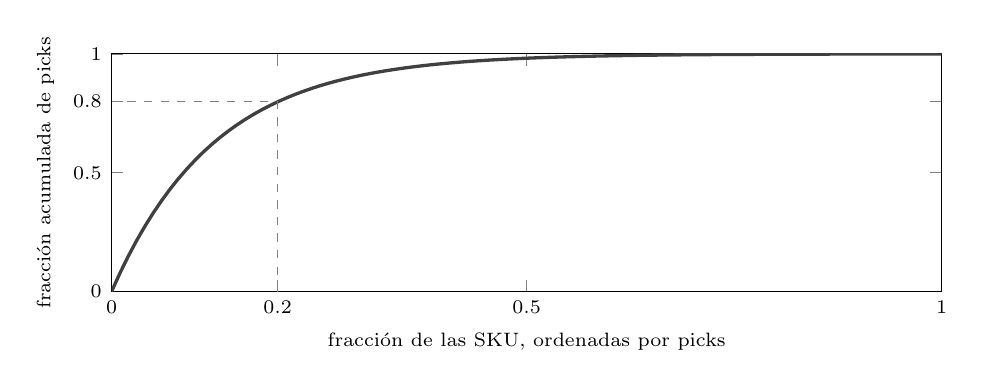
\begin{tikzpicture}
            \begin{axis}[width=\linewidth, height=4.6cm, xlabel={fracción de las SKU, ordenadas por picks}, ylabel={fracción acumulada de picks}, xmin=0, xmax=1, ymin=0, ymax=1, xtick={0,0.2,0.5,1}, ytick={0,0.5,0.8,1}, tick label style={font=\scriptsize}, label style={font=\scriptsize}, grid=none]
                \addplot[very thick, black!75, domain=0:1, samples=100] {(1-exp(-8*x))/(1-exp(-8))};
                \draw[dashed, black!50] (axis cs:0.2,0) -- (axis cs:0.2,0.8) -- (axis cs:0,0.8);
            \end{axis}
        \end{tikzpicture}
        \caption{curva de Pareto de los picks}
        \label{fig:perfil-pareto}
    \end{subfigure}
    \hfill
    \begin{subfigure}{0.48\textwidth}
        \centering
        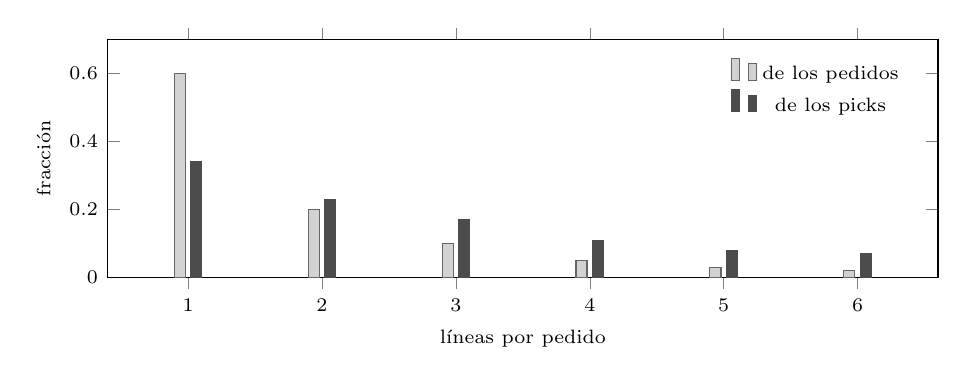
\begin{tikzpicture}
            \begin{axis}[width=\linewidth, height=4.6cm, ybar, bar width=4pt, xlabel={líneas por pedido}, ylabel={fracción}, xmin=0.4, xmax=6.6, ymin=0, ymax=0.7, xtick={1,...,6}, ytick={0,0.2,0.4,0.6}, tick label style={font=\scriptsize}, label style={font=\scriptsize}, legend style={font=\scriptsize, draw=none, at={(0.97,0.95)}, anchor=north east}]
                \addplot[fill=gray!35, draw=black!60] coordinates {(1,0.60) (2,0.20) (3,0.10) (4,0.05) (5,0.03) (6,0.02)};
                \addplot[fill=black!70, draw=black!70] coordinates {(1,0.34) (2,0.23) (3,0.17) (4,0.11) (5,0.08) (6,0.07)};
                \legend{de los pedidos, de los picks}
            \end{axis}
        \end{tikzpicture}
        \caption{distribución de líneas por pedido}
        \label{fig:perfil-lineas}
    \end{subfigure}
    \caption{Dos vistas esquemáticas del perfil de actividad. En (a) una fracción chica de las SKU concentra la mayor parte de los picks, y en (b) los pedidos de una línea son la mayoría pero aportan una parte menor del trabajo.}
    \label{fig:perfil}
\end{figure}

Así mismo, el propo perfil también cambia con el tiempo,
casi todo producto tiene cierta estacionalidad, ya sea anual, mensual o semanal, y no siempre es el obvia, y a eso se suman las SKU nuevas, que aparecen poco pedidas solo porque llevan poco tiempo almacenadas.
Hay además una asimetría que surge de la propia forma de la curva, mientras el tramo de las SKU más pedidas es estable, y una que fue muy pedida el mes pasado suele seguir siéndolo el siguiente, en la cola es imposible saber si una SKU se va a pedir, y con cantidades tan chicas cualquier fluctuación parece una tendencia.

Todo lo anterior mide cada SKU de forma individual, pero los pedidos con varias líneas tienen otra información, qué cosas se piden juntas.
El paso más simple es contar, para cada par de familias de productos, en cuántos pedidos aparecen las dos, y con eso ya se ve, por ejemplo, que casi todo pedido que trae algo de una familia trae también algo de otra, lo que sugiere guardarlas cerca \citep[capítulo~14]{bartholdi2014warehouse}.
Ese conteo esconde una trampa, porque dos familias pueden coincidir pocas veces en total y sin embargo una de ellas casi nunca pedirse sin la otra.
Con pares el trabajo es manejable, con ternas y más crece tan rápido que deja de serlo.
Las dos miradas sirven para cosas distintas, y las secciones que siguen las toman por separado, primero la asignación de ubicaciones a partir de lo que se sabe de cada SKU y después la afinidad a partir de lo que se sabe de sus pares.

\section{Asignación de ubicaciones}
\label{sec:slotting}

La geometría dice qué ubicaciones valen más y el perfil dice qué SKU se piden más, y la asignación de ubicaciones, o slotting, es juntar las dos cosas, decidir qué SKU va en cada ubicación.
A diferencia del edificio y del equipo, es una decisión que se toma sobre un depósito ya armado y que se puede volver a tomar cuando la demanda cambia, lo que la hace la más barata de corregir de todas las vistas hasta acá.
Esta sección recorre las reglas con que se la resuelve, de la más simple a la que usa el historial de picks.

Hay dos niveles de decisión.
El primero es si cada SKU tiene un lugar fijo, a lo que se llama almacenamiento dedicado, o si puede guardarse en cualquier ubicación libre, lo que se conoce como almacenamiento compartido.
El compartido aprovecha bien el espacio, porque una ubicación que se vacía vuelve a usarse enseguida, pero dispersa cada producto por el depósito y su ubicación cambia todo el tiempo, así que exige un WMS que sepa dónde está cada cosa y disciplina para no sacarla de otro lado.
El dedicado, en cambio, deja que los operarios aprendan el layout y que lo más pedido se ponga cerca, a cambio de que sus ubicaciones queden parcialmente vacías durante buena parte del ciclo, porque se llenan al reponer y se van vaciando hasta la siguiente reposición.
En el caso más sencillo e idealizado, con consumo constante y reposición al vaciarse, una ubicación que recibe $Q$ unidades por ciclo de largo $T$ tiene un stock $I(t) = Q\,(1 - t/T)$, cuyo promedio es
\begin{equation}
    \frac{1}{T}\int_0^T Q\left(1 - \frac{t}{T}\right)\,dt = \frac{Q}{2},
    \label{eq:diente-sierra}
\end{equation}
es decir que la mitad del espacio reservado está ocioso en promedio, como muestra la Figura~\ref{fig:diente-sierra}, y esa fracción cambia si la demanda es irregular, si se repone antes de vaciar o si se guarda stock de seguridad.

\begin{figure}[ht]
    \centering
    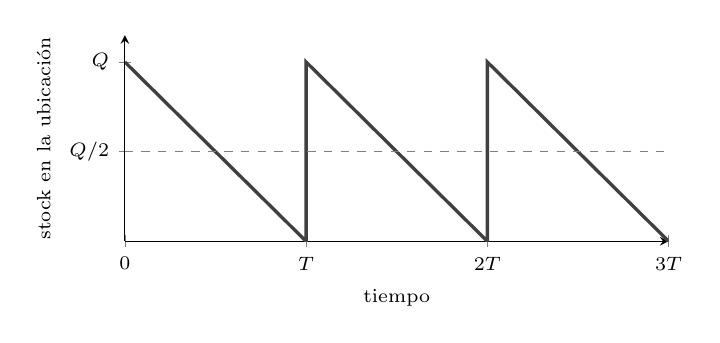
\begin{tikzpicture}
        \begin{axis}[width=0.7\textwidth, height=4.2cm, xlabel={tiempo}, ylabel={stock en la ubicación}, xmin=0, xmax=3, ymin=0, ymax=1.15, xtick={0,1,2,3}, xticklabels={$0$,$T$,$2T$,$3T$}, ytick={0.5,1}, yticklabels={$Q/2$,$Q$}, tick label style={font=\scriptsize}, label style={font=\scriptsize}, axis lines=left]
            \addplot[very thick, black!75] coordinates {(0,1) (1,0) (1,1) (2,0) (2,1) (3,0)};
            \addplot[dashed, black!50, domain=0:3] {0.5};
        \end{axis}
    \end{tikzpicture}
    \caption{Stock de una ubicación dedicada bajo consumo constante y reposición al vaciarse. Se llena con $Q$ unidades en cada reposición y baja en línea recta hasta cero, de modo que en promedio ocupa la mitad del espacio reservado. Adaptado de \citet[capítulo~2]{bartholdi2014warehouse}.}
    \label{fig:diente-sierra}
\end{figure}

El segundo nivel es con qué regla se elige la ubicación, y las más usadas son la aleatoria, que toma cualquier ubicación libre con igual probabilidad y reparte el tráfico por todo el depósito, la de la ubicación libre más cercana al dock, que es lo que termina pasando cuando se deja elegir al operario y que con el tiempo llena el frente y deja el fondo vacío, y las que ordenan las SKU por su actividad, por clases o una por una, que son las que usan el historial de picks.
Estas últimas piden almacenamiento dedicado, y para elegir con ellas hay que empezar por medir dos cosas, qué tan lejos queda cada ubicación del punto donde empiezan y terminan los recorridos, y cuántas veces se la va a visitar, porque el costo de una asignación sale de combinar una con la otra.

Para lo primero alcanza con la distancia, 
si los recorridos salen del dock y vuelven a él, a cada ubicación $k$ le corresponde un costo de acceso $c_k$, la distancia de ida y vuelta, que depende solo de la geometría, y la Figura~\ref{fig:conveniencia} muestra dos ubicaciones con $c_k$ distinto en un mismo layout.
Para lo segundo sirve el perfil de actividad, porque si la SKU $i$ se pide $f_i$ veces y está guardada en la ubicación $k(i)$, la caminata que genera es proporcional a $f_i\, c_{k(i)}$ y la de todo el depósito a
\begin{equation}
    \sum_i f_i\, c_{k(i)},
    \label{eq:costo-lineal}
\end{equation}
donde los $c_k$ vienen dados por el edificio, y pueden medirse de distintas maneras, en línea recta con la norma euclídea, sumando el tramo a lo largo del pasillo y el transversal con la norma uno, o como el largo del camino real entre estanterías, que es la que corresponde en un depósito porque las estanterías no se atraviesan, mientras que la asignación $k(i)$ es lo que se decide \citep[sección~6.2]{bartholdi2014warehouse}.
Si cada viaje va del dock a una sola ubicación y vuelve, el costo de cada ubicación no depende de lo que haya en las demás, y por eso la suma es fácil de minimizar.
Basta ordenar las ubicaciones de menor a mayor $c_k$, ordenar las SKU de más a menos $f_i$ y asignarlas en ese orden, y ningún otro reparto da una suma menor, porque si dos SKU quedaran en el orden contrario intercambiarlas nunca la aumenta.
Con recorridos que visitan varias ubicaciones por viaje la suma deja de ser la caminata real y pasa a ser una aproximación, porque el costo de ir a una ubicación depende de cuáles otras se visitan en el mismo recorrido, y esa diferencia vuelve a aparecer en la Sección~\ref{sec:formulacion}.

\begin{figure}[ht]
    \centering
    \begin{tikzpicture}[x=1cm, y=1cm]
        % estanterias
        \foreach \i in {0,...,7} \draw[fill=gray!25, draw=black!60] (\i*0.62, 0.5) rectangle ++(0.24, 2.4);
        % dock de recepcion abajo y de despacho arriba, al centro
        \fill[black!70] (2.29, 0.1) circle (0.07);
        \node[font=\scriptsize] at (2.29, -0.2) {recepción};
        \fill[black!70] (2.29, 3.3) circle (0.07);
        \node[font=\scriptsize] at (2.29, 3.6) {despacho};
        % ubicacion A, cerca de la linea entre los docks
        \fill[black] (2.22, 1.7) circle (0.08);
        \node[font=\scriptsize, anchor=west] at (2.3, 1.7) {$A$};
        \draw[thick, black!75, -{Stealth}] (2.29, 0.1) -- (2.29, 1.7) -- (2.29, 3.3);
        % ubicacion B, en una esquina
        \fill[black] (0.36, 2.6) circle (0.08);
        \node[font=\scriptsize, anchor=east] at (0.3, 2.6) {$B$};
        \draw[thick, black!45, dashed, -{Stealth}] (2.29, 0.1) -- (0.43, 0.3) -- (0.43, 2.6) -- (0.43, 3.1) -- (2.29, 3.3);
    \end{tikzpicture}
    \caption{Dos ubicaciones en un mismo layout. Para $A$ el viaje de recepción a despacho pasando por la ubicación es casi directo, mientras que para $B$ hay que desviarse hasta una esquina y volver, de modo que $c_A < c_B$.}
    \label{fig:conveniencia}
\end{figure}

Las $f_i$ cuentan solo uno de los dos motivos por los que se visita una ubicación,
por un lado la visitan los operarios que recolectan, una vez por cada pedido que pide esa SKU, y por el otro la visitan los que reponen, una vez por cada vez que hay que volver a llenarla, y las dos frecuencias pueden ser muy distintas.
Conviene entonces separar los picks $f_i$ de las reposiciones $r_i$, y la rotación del inventario, las unidades despachadas sobre las que se tienen en stock, es una tercera cosa, que va con $r_i$ y no con $f_i$.
Además cuando una SKU ocupa varias ubicaciones hace falta una heurística o forma de elegir desde cuál recolectar y en cuál reponer, la más cercana para caminar menos, la que tiene menos stock para liberarla antes, o la que tiene más para ir vaciándolas de forma pareja.
Cuando se mueven pallets enteros las tres medidas son la misma, porque cada pallet que entra se repone una vez y se extrae una vez, y de ahí viene la regla de guardar cerca lo que más rota.
Cuando se recolectan piezas, en cambio, lo que manda es $f_i$, y ordenar las SKU por picks no da el mismo orden que ordenarlas por rotación.
Una medida que respeta esa diferencia es el espacio que una SKU necesita dividido por la cantidad de pedidos que la piden, conocida como \emph{cube-per-order index} o COI \citep{heskett1963cube}\completar{chequear esta referencia}, que manda a las mejores ubicaciones a las SKU que dan más picks por metro ocupado.

Asignar una ubicación a cada SKU según su puesto en el ranking es lo más preciso, pero rara vez se hace así.
Lo habitual es cortar el ranking en dos o tres clases, las A, B y C del perfil, reservar una zona del depósito para cada clase y, dentro de la zona, guardar donde haya lugar.
Se pierde algo de distancia respecto de asignar una por una, pero a cambio una SKU solo se mueve cuando cambia de clase y no cada vez que cambia de puesto.
Las zonas pueden dibujarse de dos maneras, con las A ocupando el tramo de cada pasillo más cercano al corredor frontal, o con las A ocupando enteros los pasillos más cercanos al dock, y cuál conviene depende de la política de ruteo con que después se recorra.
A todo esto se le suman restricciones que el ranking no ve, como que lo pesado vaya abajo y lo liviano arriba, que lo más pedido quede a la altura de las manos, que lo que necesita frío o es peligroso tenga su zona, que cada ubicación tenga un tamaño, y que algunas familias que vienen dadas de afuera, por proveedor o por categoría, se prefiera mantenerlas juntas.

Ninguna de estas reglas se puede juzgar sola, 
la misma asignación rinde distinto según la política de ruteo con que se recorra el depósito y cuántos pedidos se junten en cada pasada, ya que asignar SKU por SKU se nota más con pedidos chicos, mientras que con la política en S y listas largas las asignaciones se parecen cada vez más entre sí, de modo que una política de almacenamiento se compara siempre con un ruteo y un batching fijos.
A eso se suma la pregunta de cuándo se decide, 
Una cosa es armar la asignación desde cero, cuando se abre un depósito o se cambia el layout, y otra es mantenerla, porque el ranking que la justificó cambia con el tiempo, entran SKU nuevas, otras dejan de pedirse y la estacionalidad mueve a las del medio, así que una asignación que fue buena se va desarmando sola.
Como mover una SKU cuesta un viaje de operario, un hueco que hay que tener libre y una actualización en el WMS, en la práctica no se reasigna todo de golpe, sino que se hace por partes, o bien se aprovecha cada reposición para guardar la SKU directamente en su lugar nuevo, y así el depósito se va corrigiendo de a poco.
Por último, poner lo más pedido cerca del dock tiene un costo escondido, porque concentra a los operarios en los mismos pasillos a la misma hora, y en un pasillo angosto uno espera al otro, de modo que las esperas se acumulan sin que la suma de distancias las vea, y por eso una asignación algo más repartida puede funcionar mejor en la práctica que la que da la cuenta.

\section{Afinidad entre productos}
\label{sec:afinidad}

La Sección~\ref{sec:perfil} terminó contando pares de familias que aparecen juntas en un mismo pedido, y esta sección baja esa cuenta al nivel de las SKU, porque la demanda de un producto no es independiente de la de los demás.
Antes de medir nada conviene distinguir cuatro terminos que se suelen usar como de forma indistinta, pero que guardan ciertas diferencias.
\textbf{Co-ocurrencia} es un conteo, de en cuántos pedidos aparecieron dos SKU cualquiera, luego 
\textbf{asociación} es dar un paso más y afirmar que cuando aparece una tiende a aparecer la otra, lo que se escribe como una regla de $i$ hacia $j$ y se evalúa con dos números, qué tan seguido se da el par y, de las veces que se pidió $i$, en cuántas también se pidió $j$, por otro lado la
\textbf{correlación} es relacion estadística, cuánto se aleja lo que se pidió junto de lo que se esperaría si las dos demandas fueran independientes, la misma puede ser negativa, así como dos SKU muy pedidas pueden coincidir mucho sin estar correlacionadas, finalmente la
\textbf{Afinidad} es el término que se usa en la literatura de slotting para el peso que dice cuánto conviene guardar dos SKU cerca, no se trata un dato sino una decisión, porque se construye con alguna de las tres anteriores.

Lo segundo que hay que fijar es qué quiere decir que dos SKU van juntas, y la opción más común es el pedido del cliente, dos SKU van juntas si alguien las compró en la misma orden.
Pero el operario no camina un pedido, camina una lista de recolección, y cuando hay batching esa lista junta varios pedidos, y una \emph{wave} junta varias listas que salen en el mismo camión.
Por eso comprados juntos y recolectados juntos son dos cosas distintas, dos SKU que ningún cliente pidió a la vez podrían aparecer de forma recurrente en la misma lista, aunque sea poco probable, y dos que casi siempre se compran juntas podrían quedar repartidas en listas separadas.
Si lo que se quiere bajar es la caminata, lo que corresponde es contar sobre la lista, que es lo que el operario recorre, y usar el pedido solo cuando cada lista es un pedido o cuando se comprueba que las dos cuentas dan parecido, algo que depende de cómo el algoritmo de batching arma las listas.

Con eso fijado, todas las medidas se arman con los mismos cuatro números, la cantidad $N$ de pedidos, la frecuencia o soporte $s_i$ y $s_j$ de cada SKU, es decir en cuántos pedidos aparece cada una, y la co-ocurrencia $n_{ij}$, en cuántos aparecen las dos, y la Tabla~\ref{tab:medidas-afinidad} reúne algunas de las más usadas.
La co-ocurrencia y el soporte del par cuentan lo mismo, el segundo dividido por $N$, y las dos favorecen a los pares populares, porque dos SKU muy pedidas coinciden mucho aunque no tengan nada que ver entre sí.
La confianza es la única de las presentadas que es asimétrica, dice qué fracción de los pedidos de $i$ trae también a $j$, que es la probabilidad condicional $P(j \mid i)$ estimada del historial, y puede ser alta de $i$ a $j$ y baja al revés cuando una es mucho más pedida que la otra.
El lift compara las coincidencias observadas con las que se esperarían si las dos SKU fueran independientes, y esas esperadas salen de multiplicar la probabilidad de que un pedido traiga a $i$, que es $s_i/N$, por la de que traiga a $j$, y de volver a multiplicar por los $N$ pedidos, lo que da $s_i s_j / N$.
Vale 1 cuando lo observado es lo esperado, más de 1 cuando van juntas más de lo que daría el azar y menos de 1 cuando se evitan, así que es la más cercana a la idea de correlación, pero con soportes chicos se dispara, porque dos SKU pedidas tres veces cada una entre 10.000 pedidos tienen menos de una milésima de coincidencia esperada, y una sola coincidencia real ya da un lift de más de mil, que es justamente el régimen de la cola larga \citep{li2015dynamic}.
Jaccard mira, de todos los pedidos que trajeron a alguna de las dos, qué fracción trajo a las dos, y el coseno hace algo parecido dividiendo por la media geométrica de los soportes, y por eso las dos suben a los pares raros que casi siempre van juntos y bajan a los populares que coinciden mucho pero en una fracción chica de sus pedidos, y en la literatura de slotting Jaccard es la elección más frecuente, por convención más que por derivación \citep{zhang2016correlated}.

\begin{table}[ht]
    \centering
    \small
    \renewcommand{\arraystretch}{1.6}
    \begin{tabularx}{\textwidth}{|l|c|c|L|}
        \hline
        \textbf{Medida} & \textbf{Fórmula} & \textbf{Rango} & \textbf{Qué premia} \\
        \hline
        Co-ocurrencia & $n_{ij}$ & $0$ a $\min(s_i, s_j)$ & pares populares que coinciden mucho \\
        \hline
        Soporte del par & $\dfrac{n_{ij}}{N}$ & $0$ a $1$ & lo mismo, como fracción de los pedidos \\
        \hline
        Confianza de $i$ a $j$ & $\dfrac{n_{ij}}{s_i}$ & $0$ a $1$ & que $j$ acompañe a $i$, sin importar cuánto se pide $j$ \\
        \hline
        Lift & $\dfrac{N\,n_{ij}}{s_i\,s_j}$ & $0$ a $N$ & exceso sobre la independencia, uno si no hay relación \\
        \hline
        Jaccard & $\dfrac{n_{ij}}{s_i + s_j - n_{ij}}$ & $0$ a $1$ & pares que casi siempre van juntos \\
        \hline
        Coseno & $\dfrac{n_{ij}}{\sqrt{s_i s_j}}$ & $0$ a $1$ & parecido a Jaccard, menos severo si $s_i$ y $s_j$ difieren \\
        \hline
    \end{tabularx}
    \caption{Medidas de relación entre dos SKU a partir de $N$ pedidos, los soportes $s_i$ y $s_j$ y la co-ocurrencia $n_{ij}$.}
    \label{tab:medidas-afinidad}
\end{table}

Que estas medidas no necesariamente responden a la misma pregunta puede verse con dos pares.
Supongamos que tenemos 10.000 pedidos, dos SKU populares $A$ y $B$, con soportes de 2.000 y 1.500 que coinciden en 300 pedidos, y dos SKU no tan populares $C$ y $D$, con soportes de 12 y 10 que coinciden en 9.
Siguiendo el orden de la tabla, por co-ocurrencia el par popular vale 300 y el otro 9, y por soporte del par 0,03 y 0,0009, de modo que las dos medidas absolutas favorecen al popular.
La confianza de $A$ hacia $B$ es 0,15 y la de $C$ hacia $D$ es 0,75, el lift del par popular es exactamente 1, porque las 300 coincidencias son justo las que se esperarían por azar, mientras que el del otro es 750, y por Jaccard y coseno el popular vale 0,09 y 0,17 contra 0,69 y 0,82 del otro, así que todas las medidas normalizadas dan vuelta el orden.
Si esos valores se usan como peso $a_{ij}$ para decidir qué acercar, con co-ocurrencia se acercan $A$ y $B$ y se ahorra caminata en 300 pedidos, mientras que con cualquiera de las otras se acercan $C$ y $D$ y se ahorra en 9.
No son entonces dos versiones de un mismo objetivo sino dos objetivos distintos, uno cuenta viajes conjuntos y el otro qué tan exclusiva es la relación, y elegir el peso es elegir qué se está minimizando.

Todo lo anterior mira de a dos SKU por vez, y esa es la simplificación más común de la literatura, porque la cantidad de pares ya crece de forma cuadrática con la cantidad de SKU y la de ternas o grupos mayores explota, aunque existen algoritmos que encuentran los conjuntos de productos que aparecen juntos con frecuencia sin tener que enumerarlos todos \citep{han2004mining}.
La afinidad tampoco tendría por qué salir del historial de pedidos, en entornos de manufactura se la ha derivado de la estructura del producto, de qué piezas forman parte de un mismo conjunto, con una señal mucho más nítida que la del comercio electrónico \citep{brynzer1996storage}, e incluso podría estimarse con modelos de aprendizaje automático a partir de los atributos de los productos.
Cualquiera sea la medida y la fuente, el resultado es una matriz simétrica y rala de pesos $a_{ij}$, que es lo mismo que un grafo con una SKU en cada nodo y una arista pesada entre cada par relacionado, como el de la Figura~\ref{fig:grafo-afinidad}.
Pensarlo así ayuda en dos cosas, porque quedarse solo con los vecinos más fuertes de cada SKU, que es lo habitual para que la matriz sea manejable, es podar aristas, y porque los métodos que agrupan productos antes de asignarlos, que se ven en la Sección~\ref{sec:estado}, buscan en ese grafo los grupos densos, como el de la izquierda de la figura, y los separan de los pares sueltos y de las SKU que no se relacionan con nadie.

\begin{figure}[ht]
    \centering
    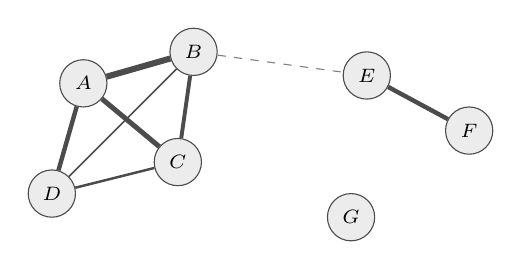
\begin{tikzpicture}[x=1cm, y=1cm, nodo/.style={circle, draw=black!70, fill=gray!15, minimum size=6mm, inner sep=0pt, font=\scriptsize}]
        % grupo denso
        \node[nodo] (a) at (0, 1.2) {$A$};
        \node[nodo] (b) at (1.4, 1.6) {$B$};
        \node[nodo] (c) at (1.2, 0.2) {$C$};
        \node[nodo] (d) at (-0.4, -0.2) {$D$};
        \draw[line width=2.2pt, black!70] (a) -- (b);
        \draw[line width=1.8pt, black!70] (a) -- (c);
        \draw[line width=1.4pt, black!70] (b) -- (c);
        \draw[line width=1.6pt, black!70] (a) -- (d);
        \draw[line width=0.9pt, black!70] (c) -- (d);
        \draw[line width=0.6pt, black!70] (b) -- (d);
        % par suelto
        \node[nodo] (e) at (3.6, 1.3) {$E$};
        \node[nodo] (f) at (4.9, 0.6) {$F$};
        \draw[line width=1.6pt, black!70] (e) -- (f);
        % union debil entre grupo y par
        \draw[line width=0.4pt, black!50, dashed] (b) -- (e);
        % SKU aislada
        \node[nodo] (g) at (3.4, -0.5) {$G$};
    \end{tikzpicture}
    \caption{Un grafo de afinidad, cada nodo es una SKU y el grosor de cada arista es el peso $a_{ij}$ del par.}
    \label{fig:grafo-afinidad}
\end{figure}


\section{Formulación matemática}
\label{sec:formulacion}
Las herramientas para escribir y resolver estas decisiones vienen de la optimización lineal, 
un programa lineal busca el mínimo de una función lineal de las variables sujeta a restricciones también lineales, y su propiedad central es que la región factible es un poliedro y el óptimo, si existe, está en alguno de sus vértices, de modo que alcanza con recorrer vértices para dar una solución.
Eso es lo que hace el método símplex, que desde que Dantzig lo propuso en 1947 resuelve en la práctica problemas con miles de variables \citep{dantzig1963linear}\completar{chequear esta referencia}.
Cuando las variables tienen que ser enteras, como cuando deciden si una SKU va o no a una ubicación, el problema se vuelve en general mucho más difícil, porque los vértices del poliedro relajado ya no son enteros y hay que buscar entre las soluciones enteras con métodos de ramificación, salvo en algunas familias afortunadas en las que la relajación alcanza.

La suma de la Ecuación~\ref{eq:costo-lineal} se puede escribir como un problema de asignación.
Con $I$ el conjunto de SKU y $L$ el de ubicaciones, la variable $x_{i\ell}$ vale 1 si la SKU $i$ va a la ubicación $\ell$ y 0 si no, y el problema es
\begin{equation}
    \begin{aligned}
        \min_{x} \quad & \sum_{i \in I} \sum_{\ell \in L} f_i\, c_\ell\, x_{i\ell} \\
        \text{sujeto a} \quad & \sum_{\ell \in L} x_{i\ell} = 1 \quad \forall i \in I \\
        & \sum_{i \in I} x_{i\ell} \le 1 \quad \forall \ell \in L \\
        & x_{i\ell} \in \{0, 1\},
    \end{aligned}
    \label{eq:asignacion-lineal}
\end{equation}
donde la primera restricción dice que cada SKU ocupa exactamente una ubicación, que es el caso del almacenamiento dedicado con un solo lugar por SKU, y si alguna necesita varias se la trata como varias copias, la segunda que cada ubicación aloja a lo sumo una SKU, con lo que puede haber ubicaciones vacías, y la tercera que la decisión es sí o no.
El costo de poner a $i$ en $\ell$ es $f_i\, c_\ell$ y no depende de dónde estén las demás, así que el objetivo es lineal en las $x_{i\ell}$, y el problema es uno de los clásicos de la investigación de operaciones, el problema de asignación.
Es además una de esas familias afortunadas, porque si se relaja la última restricción y se deja que las variables tomen cualquier valor entre 0 y 1, la solución óptima del programa lineal sigue siendo entera, así que se resuelve de forma exacta con el símplex o con algoritmos propios como el húngaro \citep{kuhn1955hungarian}\completar{chequear esta referencia}, y en este caso ni siquiera hace falta, porque el orden por $f_i$ y por $c_\ell$ de la Sección~\ref{sec:slotting} da directamente la solución óptima.

La afinidad rompe esa independencia, porque si conviene que $i$ y $j$ estén cerca, lo que cuesta poner a $i$ en $\ell$ depende de dónde haya quedado $j$.
Con $d_{\ell k}$ la distancia entre las ubicaciones $\ell$ y $k$, cada par $(i, j)$ paga su afinidad multiplicada por la distancia entre las ubicaciones que recibieron, y sumando sobre todos los pares queda
\begin{equation}
    \sum_{i \in I} \sum_{j \in I} \sum_{\ell \in L} \sum_{k \in L} a_{ij}\, d_{\ell k}\, x_{i\ell}\, x_{jk},
    \label{eq:termino-cuadratico}
\end{equation}
donde cada término lleva el producto de dos variables, $x_{i\ell}$ y $x_{jk}$, y por eso se lo llama cuadrático.
Ahí está todo el cambio, ya no alcanza con ordenar dos listas, porque mover una SKU cambia el costo de todas las que tienen afinidad con ella, y una mejora local puede empeorar el total.

Juntar los dos términos da el problema completo,
\begin{equation}
    \begin{aligned}
        \min_{x} \quad & \sum_{i \in I} \sum_{\ell \in L} f_i\, c_\ell\, x_{i\ell} + \sum_{i \in I} \sum_{j \in I} \sum_{\ell \in L} \sum_{k \in L} a_{ij}\, d_{\ell k}\, x_{i\ell}\, x_{jk} \\
        \text{sujeto a} \quad & \sum_{\ell \in L} x_{i\ell} = 1 \quad \forall i \in I \\
        & \sum_{i \in I} x_{i\ell} \le 1 \quad \forall \ell \in L \\
        & x_{i\ell} \in \{0, 1\},
    \end{aligned}
    \label{eq:qap}
\end{equation}
que es la forma que Koopmans y Beckmann le dieron en 1957 al problema de ubicar plantas industriales, con un costo de instalar cada planta en cada sitio, un flujo de mercadería entre cada par de plantas y una distancia entre cada par de sitios, y que se conoce como problema de asignación cuadrática \citep{koopmans1957assignment}.
En el slotting los papeles son los mismos, las SKU son las plantas, las ubicaciones son los sitios, la afinidad $a_{ij}$ hace de flujo y el término lineal es el de la Ecuación~\ref{eq:asignacion-lineal}, así que un problema planteado hace casi setenta años describe el de esta tesis, y la formulación propia, con qué es cada uno de esos símbolos en el depósito estudiado, se escribe en el capítulo siguiente\completar{ref al capitulo cuando exista}.

El precio de esa generalidad es la dificultad, porque el problema de asignación cuadrática es NP-hard \citep{sahni1976pcomplete}\completar{chequear esta referencia}, lo que quiere decir que pertenece a la clase de problemas para los que no se conoce ningún algoritmo cuyo tiempo crezca de forma polinomial con el tamaño de la instancia, y que si alguien encontrara uno lo tendría para todos los demás problemas de esa clase, algo que se considera muy improbable.
En la práctica eso significa que el tiempo de cualquier método exacto crece de forma exponencial, y como a diferencia de la asignación lineal la relajación no da soluciones enteras, no hay atajo, de modo que los métodos exactos como \emph{branch and bound} \citep{land1960automatic}\completar{chequear esta referencia}, que recorren el árbol de asignaciones posibles acotando el costo de cada rama y descartando las que no pueden mejorar la mejor solución conocida, dejan de terminar en tiempo razonable con apenas treinta objetos \citep{loiola2007qap}.
Para tener una idea de la escala, treinta SKU en treinta ubicaciones ya son más de $10^{32}$ asignaciones posibles, mientras que un depósito real tiene decenas de miles de cada una.
La literatura mide entonces la calidad de lo que sí se puede calcular contra dos referencias, la biblioteca QAPLIB de instancias con soluciones conocidas y la cota inferior de Gilmore y Lawler \citep{gilmore1962optimal, lawler1963quadratic}\completar{chequear estas referencias}, que sale de resolver problemas de asignación lineal y da un piso que ninguna solución puede bajar, aunque las dos sirven solo en instancias chicas.

Por eso, en la escala de un depósito, la solución exacta queda descartada y lo que se usa son heurísticas, que buscan soluciones buenas sin garantía de que sean las mejores, y la revisión de Loiola y otros las ordena en unas pocas familias \citep{loiola2007qap}.
Las constructivas arman la asignación de a una SKU, eligiendo en cada paso la ubicación más barata dado lo que ya se asignó, y son rápidas pero se quedan en el primer óptimo local que encuentran.
Las metaheurísticas, como el recocido simulado, la búsqueda tabú y los algoritmos genéticos, aceptan a veces empeorar para poder escapar de esos óptimos locales, y son las más usadas en el slotting con afinidad, aunque cada una trae parámetros que hay que calibrar \citep{li2015dynamic}.
La descomposición parte el problema en dos más chicos, y en el slotting toma la forma del esquema de dos fases que domina la literatura, agrupar primero las SKU afines y asignar después los grupos, a costa de que lo que se pierde al separar las dos decisiones rara vez se mide \citep{islam2023cslap}.
Casi todas terminan con una búsqueda local por intercambios, tomar dos SKU, permutar sus ubicaciones y quedarse con el cambio si el costo baja, que es barata porque la diferencia en la Ecuación~\ref{eq:qap} se calcula sin recomputar toda la suma, y que en la práctica es lo que pule cualquier solución inicial.

\completar{PARA EL CAPITULO PROPIO, no para aca: la formulacion de la tesis es casi la de la Ecuacion eq:qap, asi que alla va la instancia concreta, que es aij, que es d y c, el peso lambda entre los dos terminos, las restricciones del deposito, y el punto de que la suma es un surrogate de la distancia real y no la distancia, a verificar por simulacion.}

\section{Estado del arte}
\label{sec:estado}

\completar{Organizado por preguntas, nunca paper por paper. (1) Historia corta de la idea, guardar juntos lo que se pide junto: repuestos para ordenes urgentes y la farmacia que agrupa cuidado capilar (L 1.2 y 8.5), el family grouping, y el esquema dominante de dos fases, agrupar y despues asignar (Islam 2023). (2) Mapa de fuentes: las dos revisiones sistematicas (Rojas Reyes 2019, Islam 2023) como mapa, no como unica base; de Koster 2007 y Gu 2007 para SLAP en general; los clasicos (Frazelle y Sharp 1989, Brynzer 1996, Mantel 2007); los recientes (Li 2015, Zhang 2016, Xu 2020, Mirzaei 2021); y BUSCAR literatura 2023-2026, porque la tesis se escribe en 2026 y hoy no hay nada posterior a 2022. (3) La revision por preguntas, una subseccion corta por cada una: que senal de afinidad usan; como agrupan; como asignan; que funcion objetivo; que metodo de resolucion; que layout; que ruteo; si hay batching; que tamano de orden; que baseline; como evaluan y con que datos, reales o sinteticos. (4) Cuidado con el tipo de sistema: Mirzaei 2021 es parts-to-picker con pods, donde el costo es cuantos contenedores se traen y no cuanto se camina; no extrapolar sus conclusiones al picker-to-parts manual sin decirlo. (5) Cuando dos trabajos dan signo distinto para el mismo efecto, no llamarlo contradiccion antes de comparar sistema, layout, ruteo, batching, tamano de orden, distribucion de demanda, metrica de afinidad y objetivo; casi siempre son regimenes experimentales distintos. (6) La critica de Mirzaei a la secuencialidad de las dos fases, como advertencia. TABLA COMPARATIVA unica pero ancha, apaisada si hace falta: sistema, escala, layout, ruteo, batching, tamano de orden, senal de afinidad, metodo, funcion objetivo, baseline, datos reales o sinteticos, mejora reportada. Con esas columnas la tabla de condiciones experimentales sobra.}

\section{Síntesis y problemas abiertos}
\label{sec:sintesis}

\completar{Cierre del capitulo, sin supuestos propios: esos van al capitulo metodologico. (1) Cuando parece rendir la afinidad, con lo empirico de la literatura: pedidos chicos y poco batching (Mantel 2007), ruteo que no atraviese todo igual (Xu 2020), curva de demanda poco sesgada (Mirzaei 2021), correlacion real y no artefacto de popularidad (Zhang 2016, techo de 2 por ciento sin correlacion plantada). (2) Las variables que condicionan su utilidad, las cuatro anteriores mas las que la literatura casi no mira: congestion por concentrar operarios, costo de re-slotting, costo de reposicion, estabilidad temporal de la demanda y de las afinidades, si los pares que van juntos hoy siguen yendo juntos en tres meses. Recordar que el signo del efecto del tamano de orden depende del tipo de sistema, y presentarlo como regimenes distintos, no como contradiccion. (3) Las simplificaciones habituales: todo por pares, datos sinteticos con correlacion plantada, slotting estatico, un solo bloque de pasillos, sin congestion, sin reposicion, y nadie contrasta la afinidad contra un modelo nulo. (4) Problemas abiertos: escala real de decenas de miles de SKU, validar que la senal supera al azar dados los soportes, afinidades dinamicas, el costo de descomponer en dos fases. (5) Donde se ubica esta tesis, en una oracion por hueco. Aca aterriza tambien el cierre que hoy esta al final de 2.2 (pendiente punto B).}
